\chapter{Literature study}
\label{chap:rel_work}

We will first examine the effectiveness of existing models on a collection of paintings from 2 different movements.
For this we will need to have a pose estimator, a style transformer and a collection of test data. 

A first method: We will first convert the test data with the style transformer to a painting and then we will apply pose estimation.
The test data will have coordinates of the joints, which we will compare with the results of the pose estimation.
However, the joints are of the original image. How do we convert those coordinates to map to the styled image? 
Problem: This method does not use any real paintings and will be susceptible to the accuracy of the style transformer.  

A second method: We can apply pose estimation to real paintings and then convert them to a realistic image with style transfer.
We can then use pose estimation to the realistic images and compare them with the style transformed results.
This will also require a way to map the results of the real painting to that of the style transformed. 
Problem: While we’re using real paintings now, the results will still depend on the accuracy of style transformer. 

A third method: We can annotate the paintings ourselves and use pose estimation to assess the pose estimation algorithms. 
Problem: We must annotate the paintings ourselves. 

\section{Human Pose estimation}
\label{sec:hpe}

\gls{HPE} aims to detect human features from input data such as images and videos.
It's an elementary part of computer vision with many applications among which are human action recognition (sign language), human tracking (surveillance), and human-computer interaction (video games).
This is an extensively researched area with a diverse range of different techniques.
This chapter will try to give an overview of all the many challenges and proposed solutions.
The focus will be on deep learning models, which have surpassed classical solutions significantly.
Specifically, around 2D monocular \gls{HPE}.\cite{Munea2020}\cite{Zheng2012}\cite{Liu2104}\cite{chen2022}

The human body has a high degree-of-freedom due to all the limbs, self-similar parts and body types, which may cause self-occlusion or rare/complex poses.
The variations in configuration are made even larger due to clothing, lighting, foreground occlusion, as well as viewing angles and truncation, among others, as shown in fig. \ref{fig:hpe_problem_complexity}.
This makes \gls{HPE} one of the most difficult tasks in computer vision.\cite{jain2014}\cite{Chen2000}

\subsection{Representation}
\label{section:representation}

An important factor in \gls{HPE} is how the pose will be represented.
Depending on the needs of the problem you can have a skeleton-base, contour-base, or volume-base solution.\ref{fig:pose_representation}\cite{Chen2000}

\subsubsection{Skeleton-based model}
The skeleton is build of a tree-structured set of key-points that represent the joints of the human body.
These can be explicitly described by their coordinates in 2D or 3D space.\cite{Toshev2014}
More suitable for a \gls{CNN} however is a heatmap which constructs a 2D Gaussian kernel around a key-point.\cite{Liu2104}\cite{SWARH}
They are easily implemented and became the dominant representation.
While the skeleton-based model is a compact and flexible representation it suffers in this aspect by not being able to hold texture or shape information.\cite{Zheng2012}

\subsubsection{Contour representation}
To capture the shape of the body parts, contour representation uses rectangles to estimate the body contours.
These methods include cardboard models\cite{Ju96} and \gls{ASMs}\cite{COOTES95} and were mainly in use in earlier \gls{HPE} methods.\cite{Chen2000}

\subsubsection{Volume representation}
Volumetric geometric shapes can also be used as a method of representation.
Earlier methods used simple shapes like cylinders, conics, and other shapes.\cite{Sidenbladh2000}
Volume representation is a 3D mesh that represents the human body.
The most used model is \gls{SMPL}, which includes natural pose-dependent deformations imitating soft-tissue dynamics.\cite{Loper2015}  
\\
\\
For the purpose of our research, a simple model is the only thing we need.
We only need to be aware of the most essential joints to label a pose.
This makes the skeleton-based model the ideal representation to work with and will be the focus of further study.

\subsection{Discriminative Methods and Generative Methods}
Before deep learning became prominent in \gls{HPE} there were already a number of different methods in use.
Some of these methods are compatible with the deep learning methods and were thus adopted.
An early distinction is between generative and discriminative methods.

\subsubsection{Generative Model}
A generative method will work with prior beliefs about the pose.
More information about this can be found in the section about representation.\ref{section:representation}
It will project the pose on the image and verify it with the image data.
If they don't comply, the pose is adjusted by minimizing an error function.\cite{Pons-Moll2011}

\subsubsection{Discriminative Model}
Discriminative methods on the other hand, try to map the pose on the image data with learned models.
There are several methods in this category, among which are the deep learning-based methods.
The deep-learning methods are further categorized by the following sections.

\subsection{Single-Person Methods}
Single-person pose estimation will try to evaluate only one pose from an image.
There are 2 major methods that are in use: regression methods and detection-based methods.

\subsubsection{Regression-based Methods}
The regression-based methods learn a network that maps all the body key-points to the image-data directly as show in \ref{fig:single_pose_estimation_regression_methods}.
The first successful deep learning model came from Toshev and Svegedy\cite{Toshev2014} and is considered the switch in paradigm from classic approaches to deep learning \gls{HPE}.
Toshev et al. uses a 7-layered model with 5 convolution layers and 2 fully-connected layers for the pose regressor, based on AlexNet for its simple but effective architecture. \cite{AlexNet}.
They then cascade the resulting found key-points of this model to itself where it refines it using the area around the key-points.
While the network is the same, the different stages will have different learned parameters.
With every stage the found key-points become more accurate.
Carreira et al.\cite{CarreiraAFM15} introduce an Iterative Error Feedback which is a self-correction using top-down feedback.
Using the image-data and a starting pose modeled as a heatmap, the model, based on GoogLeNet\cite{googlenet}, will predict an error for each key-point.
The pose is then corrected based on the error and fed back into the model as a heatmap with the image.
With each iteration it converges towards the solution instead of making the prediction in one go.

\subsubsection{Heatmap/Detection-based Methods}
The detection-based methods will first estimate the individual body parts and then assemble them to fit a human skeleton.
This is a 2-step process and the earlier models use a combination of classic techniques with the advances of deep learning.
Tompson et al.\cite{TompsonJLB14} proposed a hybrid architecture where the detection of body parts is handled by a \gls{CNN} and use a Spatial-Model bring those together.
The last step involves removing false-positives by restricting joint inter-connectivity to enforce global pose consistency.


\subsection{Multi-Person Methods}


\subsubsection{Bottom-Up Methods}

\subsubsection{Top-Down Methods}




There are several ways that the human body joints/keypoints are represented.
A first distinction is 2D and 3D

Top-Down
Regression-based, Heatmap-based, video-based, model compression-based.

Bottom-Up
One stage, two-stage


\begin{figure}
	\centering
	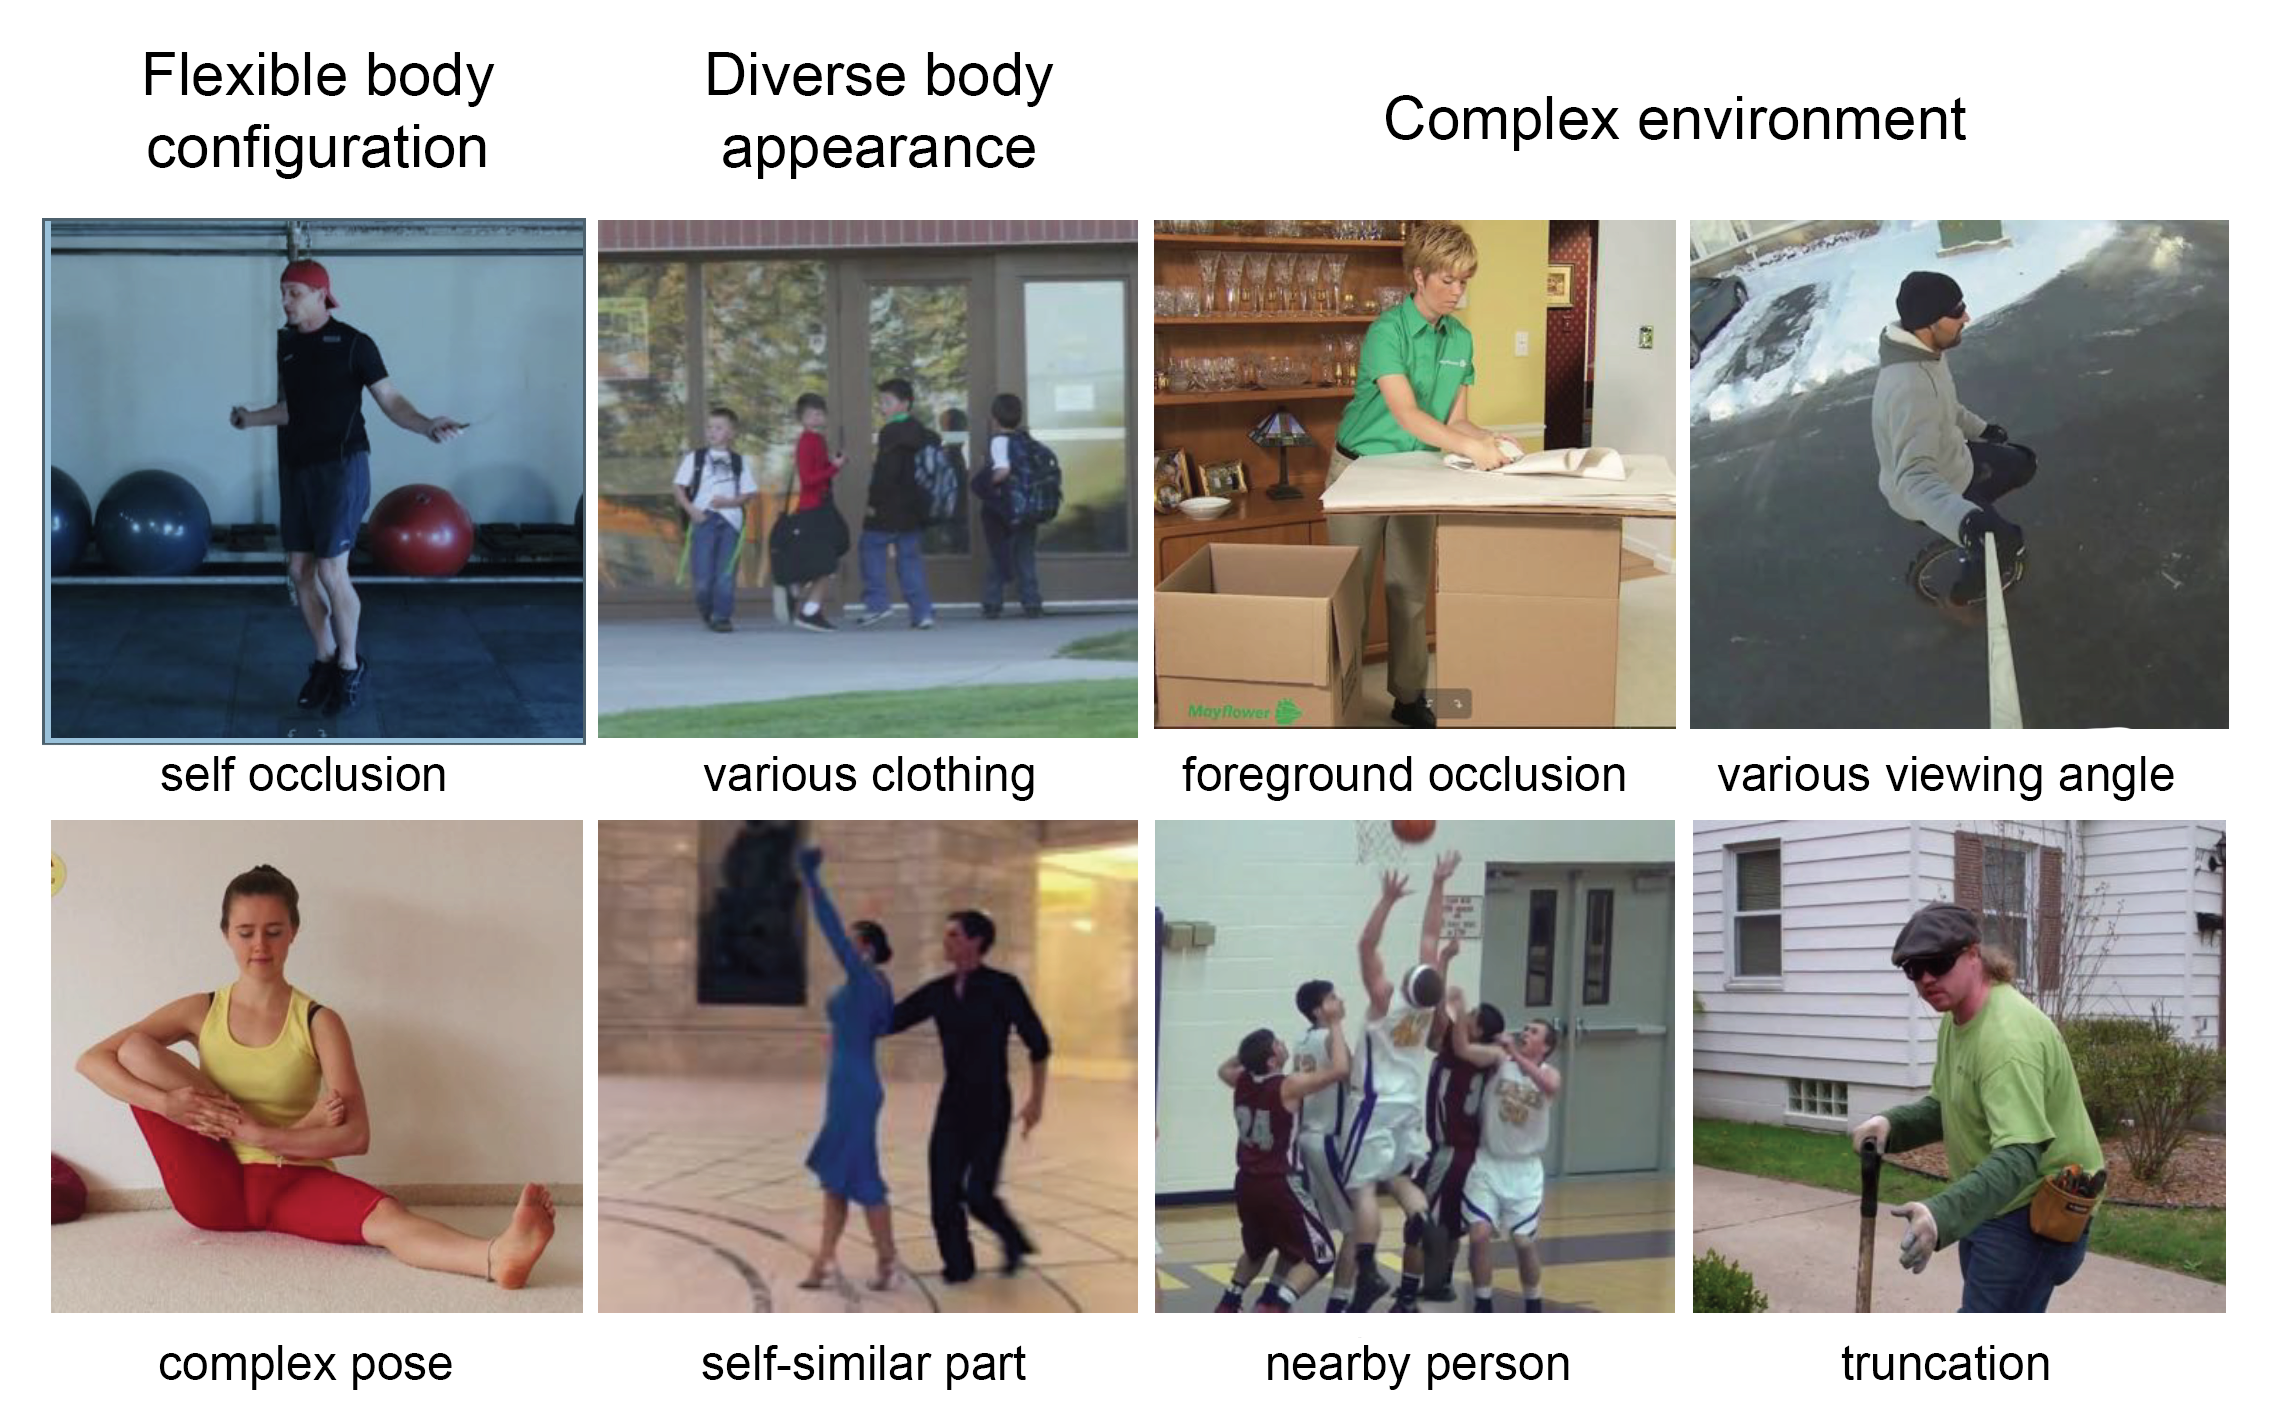
\includegraphics[width=1\textwidth]{hpe_problem_complexity}
	\caption{The various challenges HPE solutions face. Images from \gls{MPII} dataset. \cite{Andriluka2014}\cite{Chen2000}}
	\label{fig:hpe_problem_complexity}
\end{figure}

\begin{figure}
	\centering
	\subcaptionbox{Skeleton \label{fig:pose_representation_skeleton}}{%
		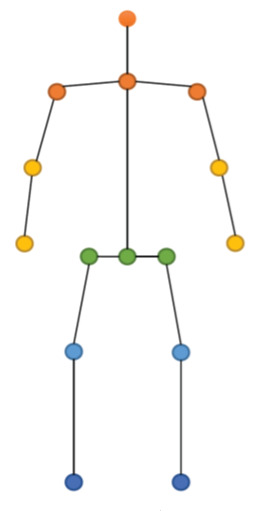
\includegraphics[width=0.3\textwidth]{pose_representation_skeleton}%
	}
	\subcaptionbox{Contour \label{fig:pose_representation_contour}}{%
		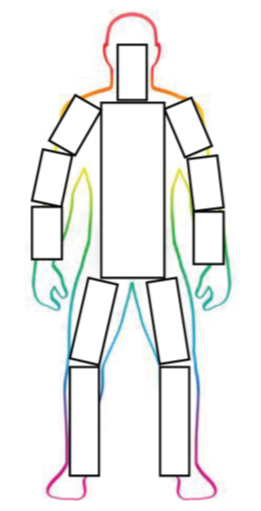
\includegraphics[width=0.3\textwidth]{pose_representation_contour}%
	}
	\subcaptionbox{Volume \label{fig:pose_representation_volume}}{%
		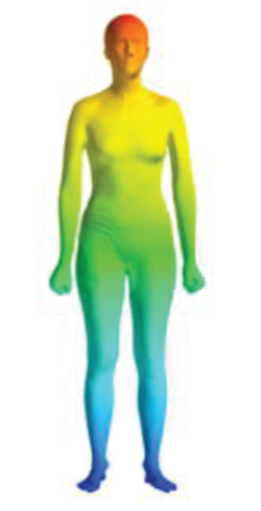
\includegraphics[width=0.3\textwidth]{pose_representation_volume}%
	}
	\caption{Models for pose representation \cite{Zheng2012}}
	\label{fig:pose_representation}
\end{figure}

\begin{figure}
	\centering
	\subcaptionbox{Regression Methods \label{fig:single_pose_estimation_regression_methods}}{%
		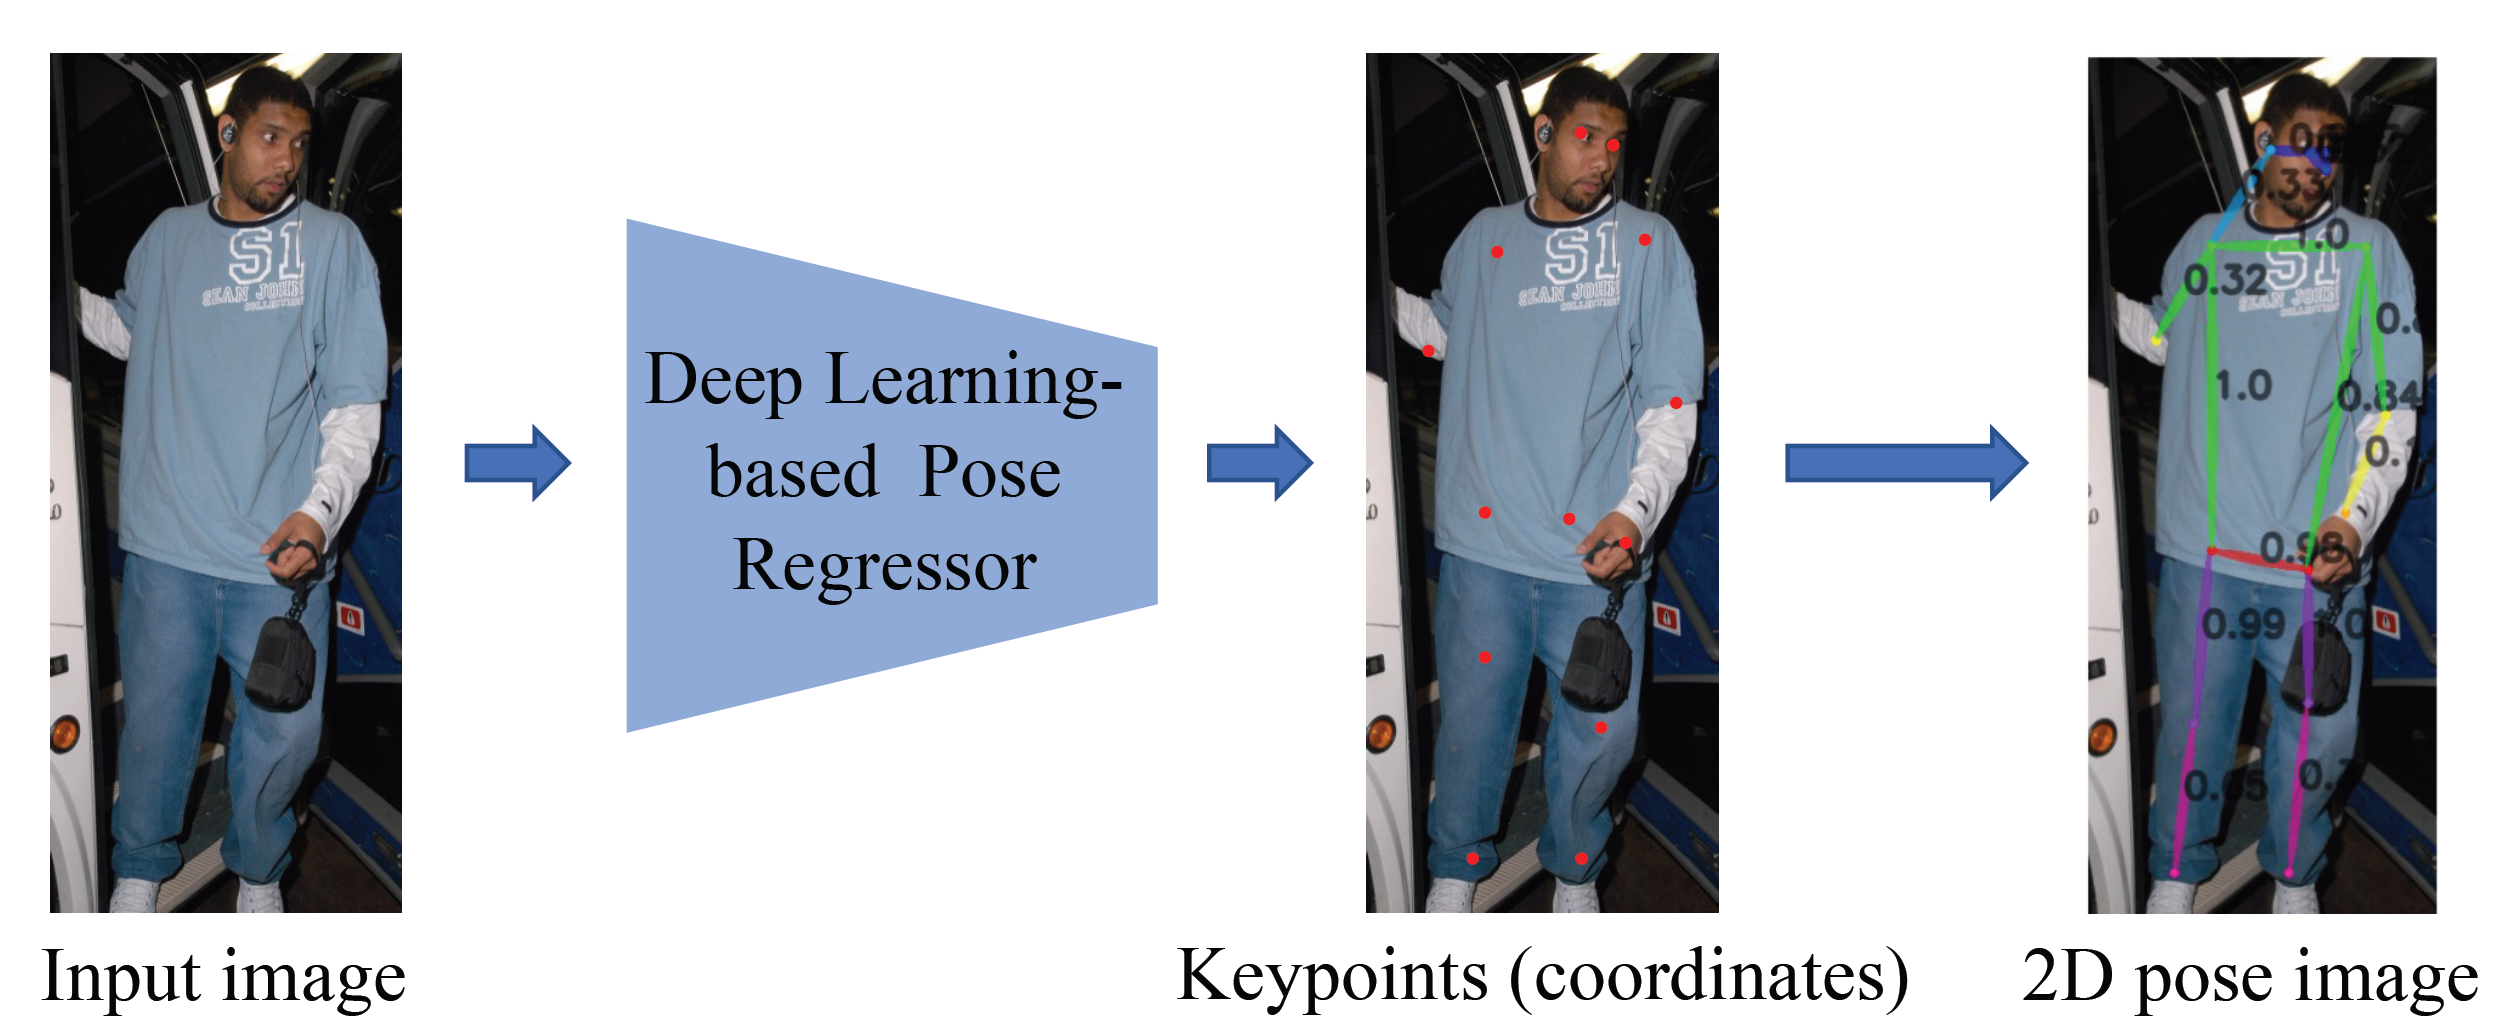
\includegraphics[width=\textwidth]{single_pose_estimation_regression_methods}%
	}
	\subcaptionbox{Heatmap-based Methods \label{fig:single_pose_estimation_heatmap-based_methods}}{%
		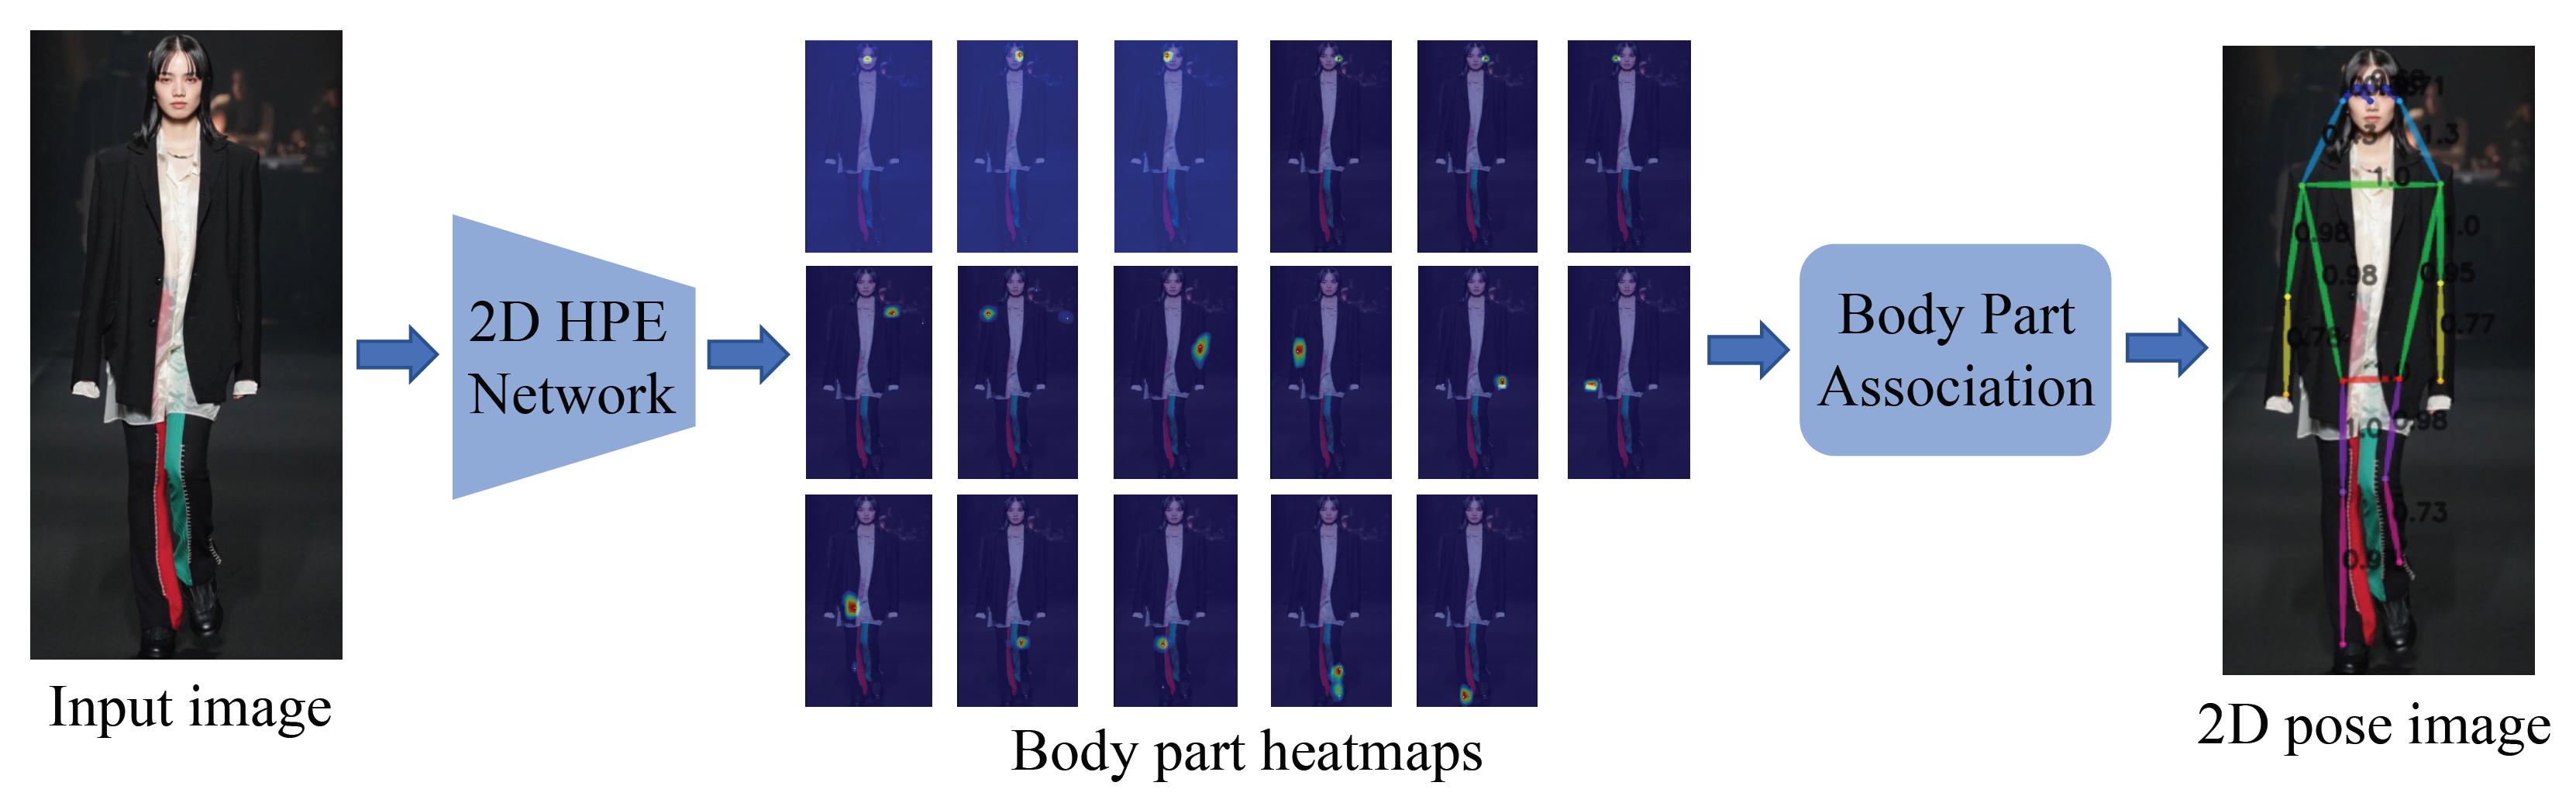
\includegraphics[width=\textwidth]{single_pose_estimation_heatmap-based_methods}%
	}
	\caption{The different methods of single-person human pose estimation.\cite{Zheng2012}}
	\label{fig:pose_representation}
\end{figure}

\begin{figure}
	\centering
	\subcaptionbox{Initial stage \label{fig:single_pose_estimation_deep_pose_initial_stage}}{%
		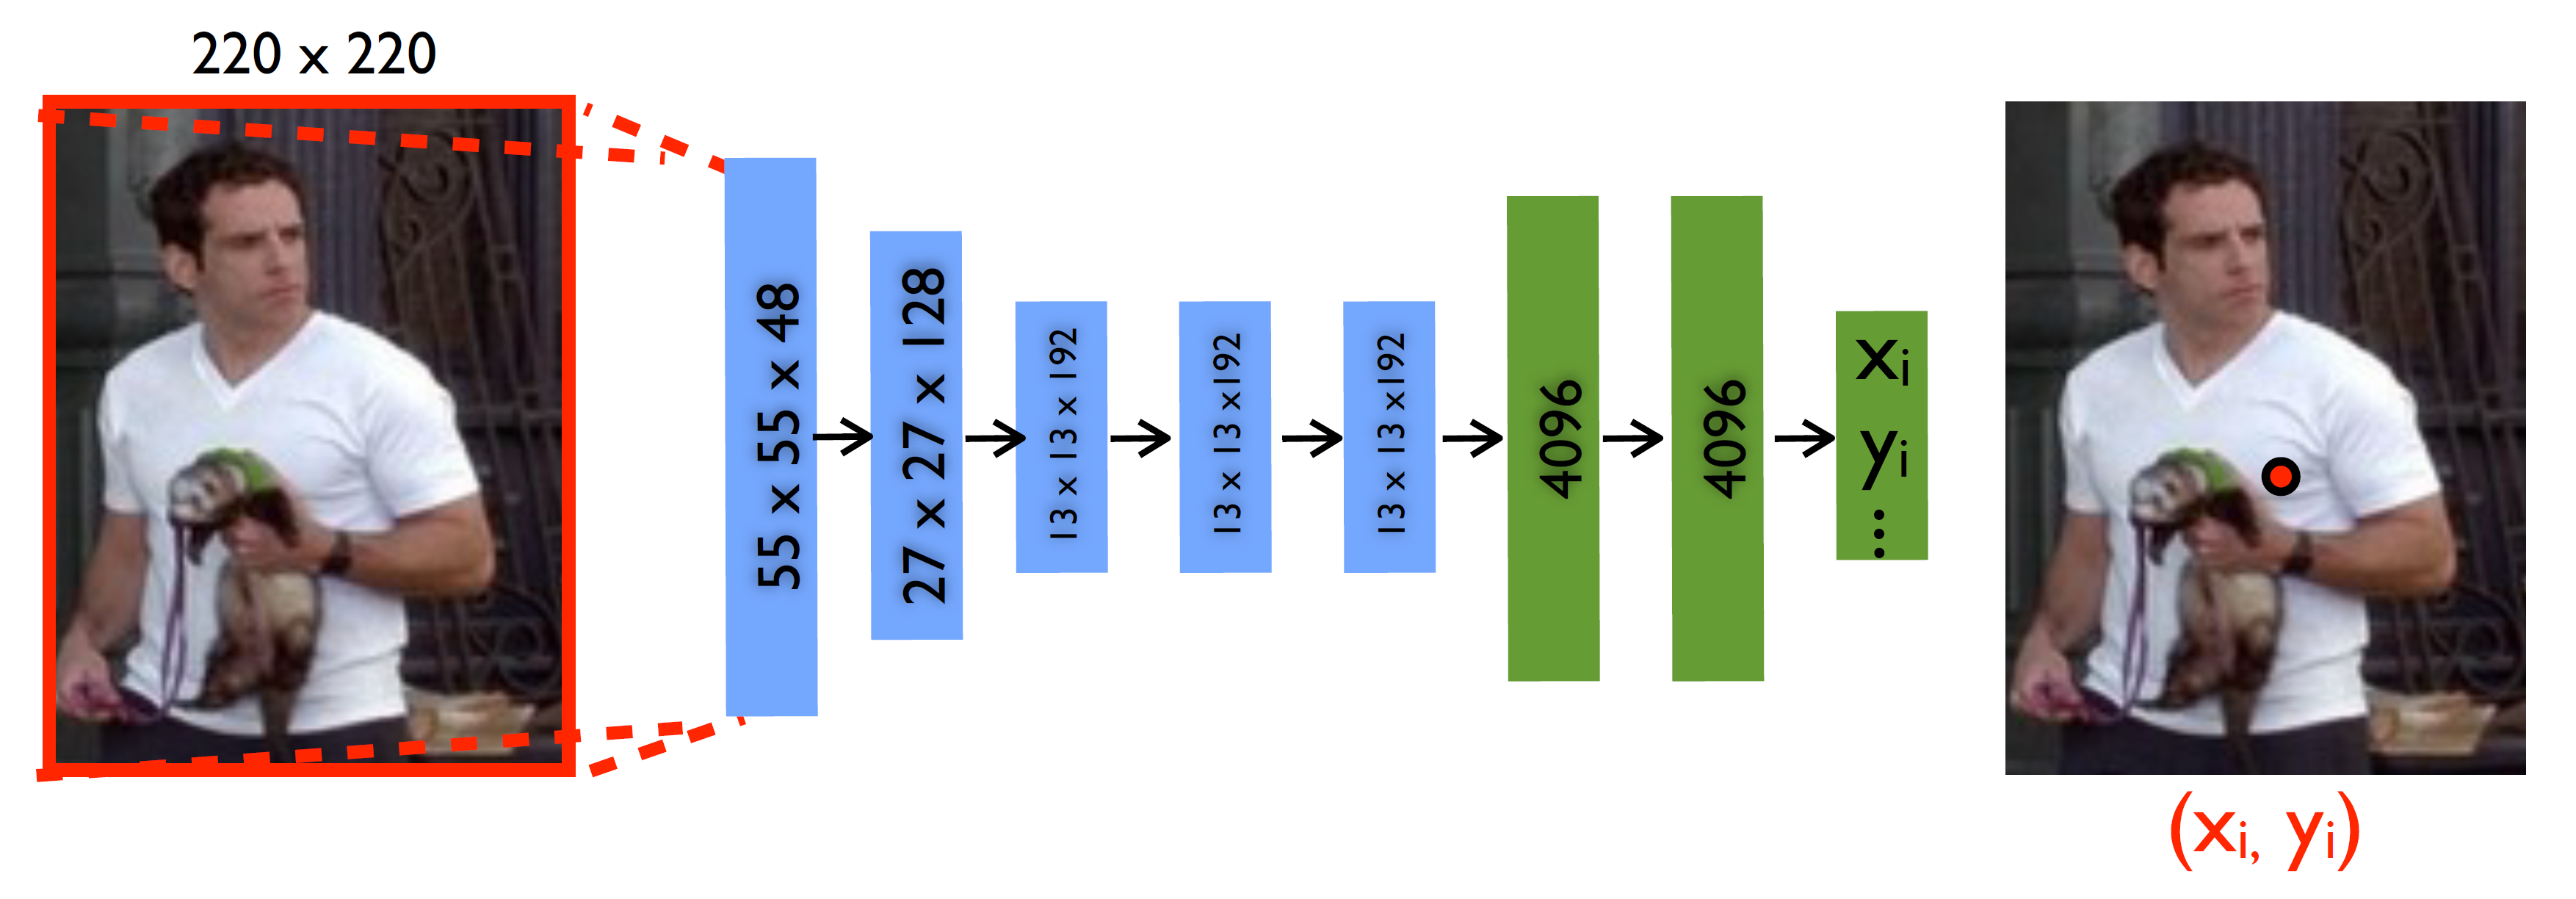
\includegraphics[width=\textwidth]{single_pose_estimation_deep_pose_initial_stage}%
	}
	\subcaptionbox{Stage s \label{fig:single_pose_estimation_deep_pose_stage_s}}{%
		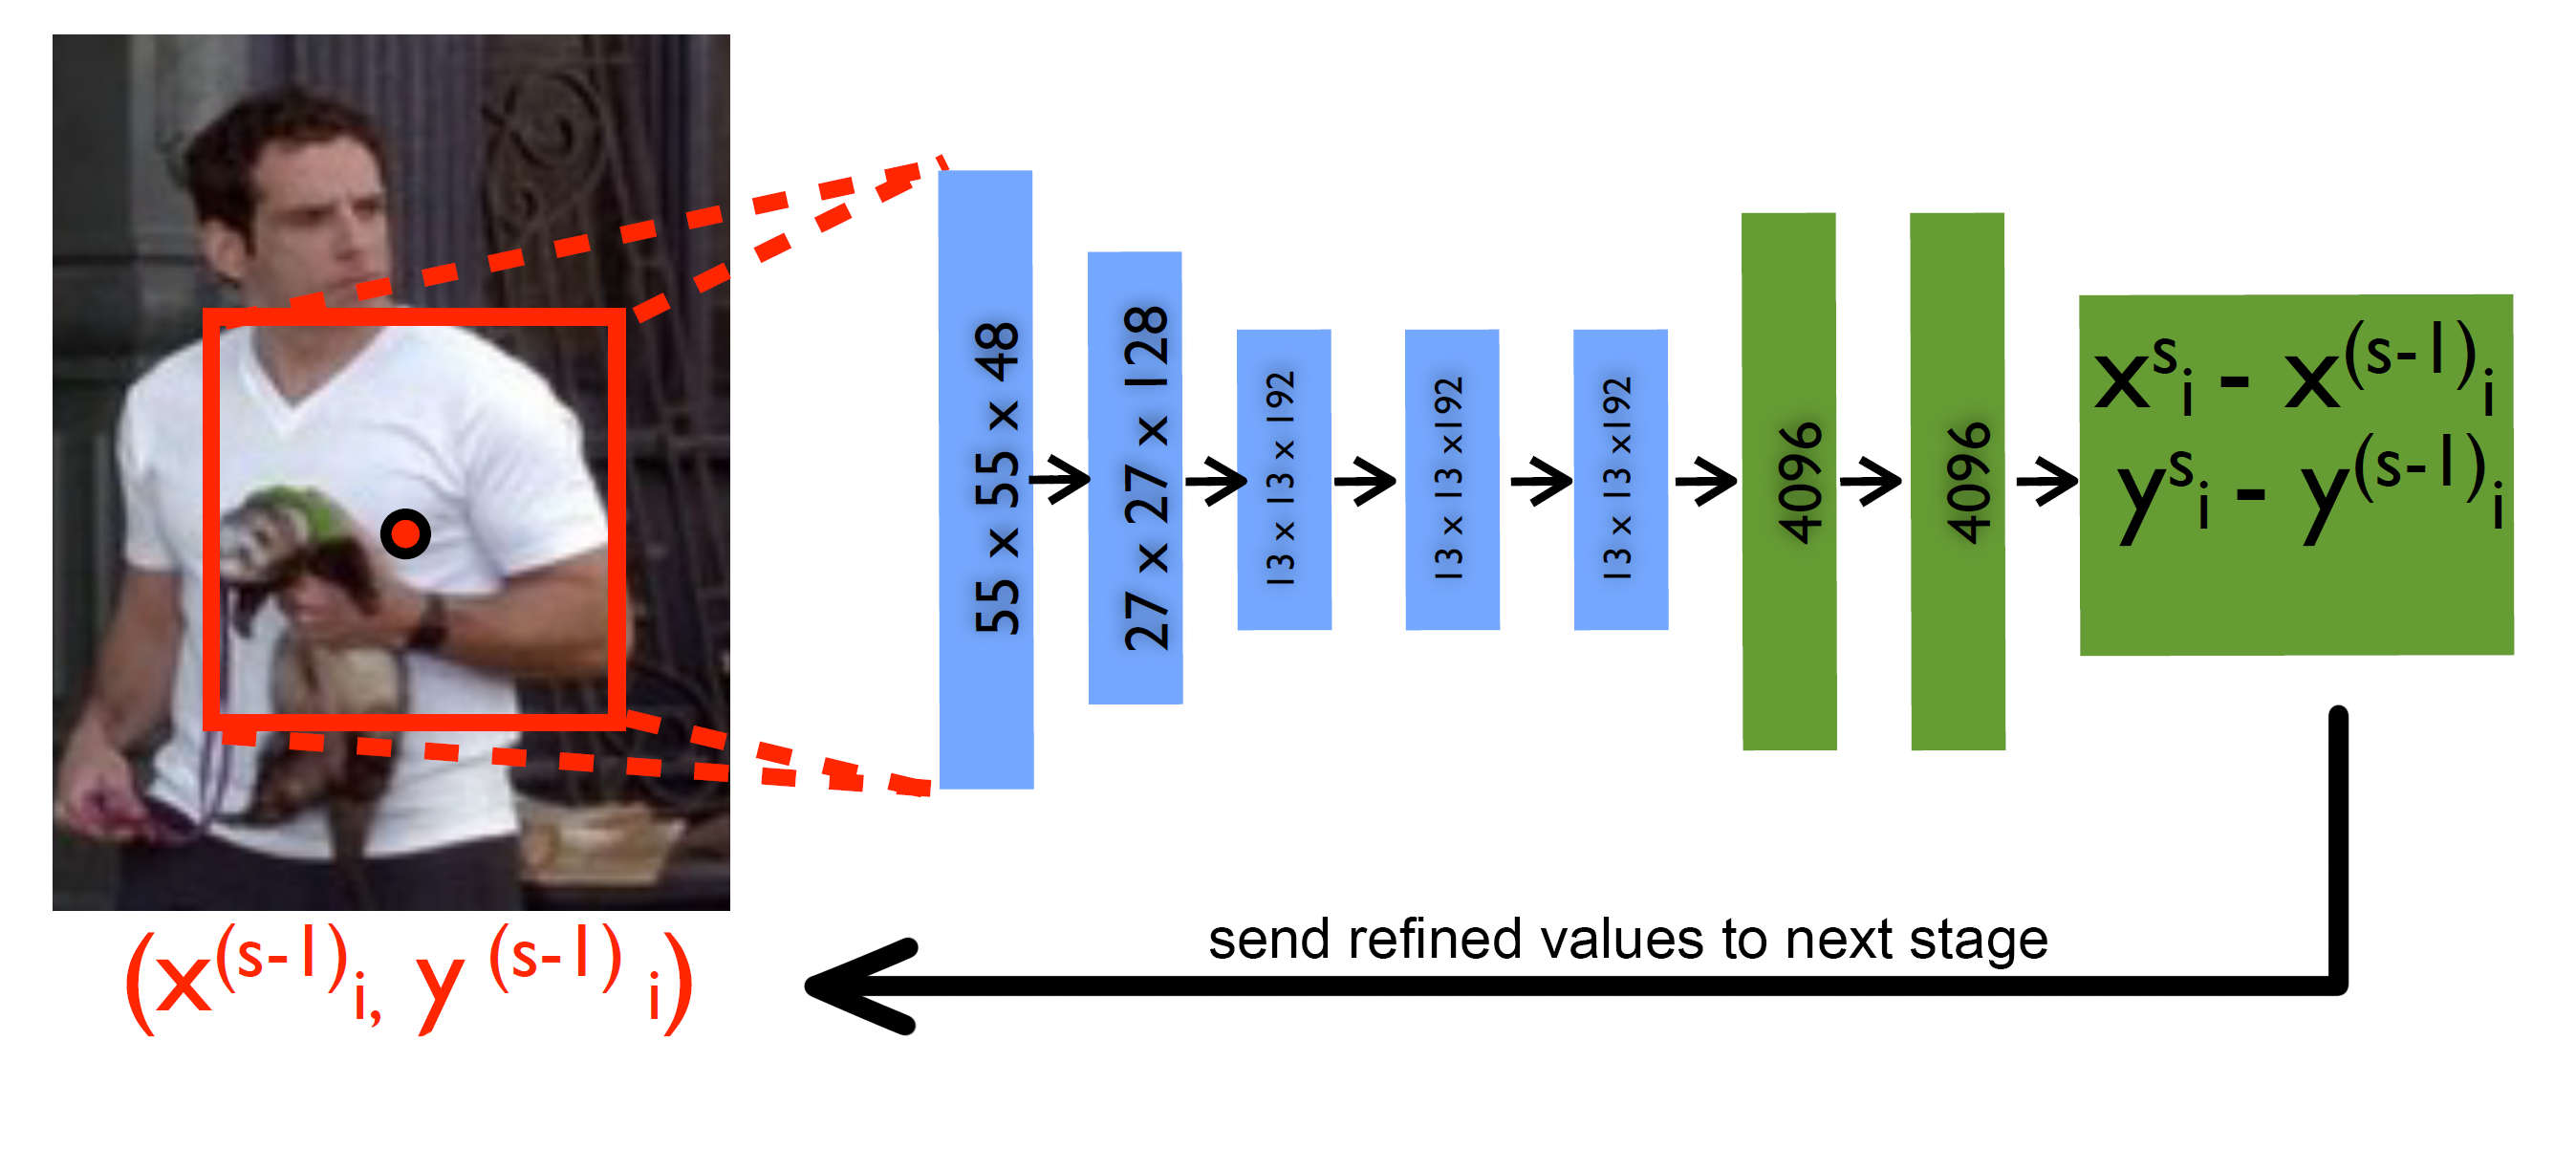
\includegraphics[width=\textwidth]{single_pose_estimation_deep_pose_stage_s}%
	}
	\caption{
		Convolution layers in blue and fully connected layers in green.
		The initial stage is applied to the whole images, while in stage s it will work on a sub-image based on the result of the previous stage.\cite{Toshev2014}
	}
	\label{fig:pose_representation}
\end{figure}

\section{Image Style Transfer}
\label{sec:ist}